Aqui será discutido a fundo o funcionamento deste dispositivo experimental que foi utilizado para o desenvolvimento das especificações HBUS.

\section{Firmware}

O firmware implementa a pilha HBUS com todas as funcionalidades. O código específico do dispositivo controla as funções de geração de PWM no microcontrolador, para acionar o circuito de controle mostrado no esquemático.

\subsection{Os objetos do dispositivo}

O código de declaração dos objetos é mostrado para exemplificar uma implementação.

\begin{minted}[linenos,fontsize=\small]{c}

const HBUSOBJ PWM_CHANNEL_0 = {{HBUSOBJ_WRITE,2,12,"PWM CANAL 00"},0x00,GET_PWM0,SET_PWM0};
const HBUSOBJ PWM_CHANNEL_1 = {{HBUSOBJ_WRITE,2,12,"PWM CANAL 01"},0x00,GET_PWM1,SET_PWM1};
const HBUSOBJ DIP_SWITCH    = {{HBUSOBJ_READ,1,6,"DIP SW"},0x00,GET_SW101,0x00};
const HBUSOBJ LDR_SENS      = {{HBUSOBJ_READ,2,10,"LDR SENSOR"},0x00,GET_LDR,0x00};
const HBUSOBJ FADE_INOUT	= {{HBUSOBJ_WRITE,4,11,"FADE IN/OUT"},0x00,GET_FADEBYTES,SET_FADEBYTES};

\end{minted}

A tabela descreve os objetos em detalhe.

\begin{table}[H]
\centering
\caption{Objetos do controlador de PWM de 2 canais}
\begin{tabular}{c c c c p{6cm}}
\hline
Objeto			&	Endereço		&	Permissão	&	Tamanho	& Descrição\\
\hline
PWM\_CHANNEL\_0	&	0x01			&	W			&	2		& Valor relativo do canal de PWM 1\\
PWM\_CHANNEL\_1 &	0x02			&	W			&	2		& Valor relativo do canal de PWM 2\\
DIP\_SWITCH		&	0x03			&	R			&	1		& Valor das chaves 1,2,3\\
LDR\_SENS		&	0x04			&	R			&	2		& Valor da leitura de luminosidade no LDR\\
FADE\_INOUT		&	0x05			&	W			&	4		& Realiza fade-in / fade-out programável\\
\hline
\end{tabular}
\end{table}

A declaração dos objetos de dispositivo:

\begin{minted}[linenos,fontsize=\small]{c}

const HBUSOBJ * MCU_OBJECTS[HBUS_OBJECT_COUNT] = {&UNIT_INFO, //obrigatorio
						&PWM_CHANNEL_0,
						&PWM_CHANNEL_1,
						&DIP_SWITCH,
						&LDR_SENS,
						&FADE_INOUT
};

\end{minted}

\subsubsection{O objeto zero}

A declaração do objeto zero e sua estrutura HBUSOBJINFO, que identifica o dispositivo é mostrada:

\begin{minted}[linenos,fontsize=\small]{c}

#define S_FAMILY 0x02000000
#define S_NUM    0x00000001

const HBUSOBJLISTINFO OBJECT_INFO = {HBUS_OBJECT_COUNT, HBUS_EP_COUNT, HBUS_INT_COUNT, 
((dword)(S_FAMILY) | (dword)(S_NUM))};
const HBUSOBJ UNIT_INFO = {{HBUSOBJ_READ,sizeof(HBUSOBJLISTINFO),12,"PWM CTRL 2CH"},
&OBJECT_INFO,0x00,0x00};

\end{minted}

\subsection{Os endpoints do dispositivo}

O dispositivo contém apenas um endpoint, que serve para o carregamento do microcódigo HBUS.

\begin{minted}[linenos,fontsize=\small]{c}
const HBUSEP EP_UCODE = {{HBUSEP_WRITE,64,9,"UCODE EP"},UCODE_IMEM,0x00,
UCODE_WRITE_IMEM_BYTE,UCODE_IMEM_WRITE_START,UCODE_IMEM_WRITE_END,0x00,0x00};
\end{minted}

Do código fonte é possível inferir que:

\begin{itemize}

\item O endpoint é de escrita apenas
\item O tamanho de bloco é 64 bytes
\item O nome do endpoint é "UCODE EP"
\item O endpoint tem funções associadas aos eventos de começo e fim de escrita

\end{itemize}

A declaração dos objetos de endpoints:

\begin{minted}[linenos,fontsize=\small]{c}

const HBUSEP * MCU_ENDPOINTS[HBUS_EP_COUNT] = {&EP_UCODE,};

\end{minted}

\subsection{As interrupções do dispositivo}

O controlador de PWM de 2 canais possui apenas a interrupção básica de erro fatal:

\begin{minted}[linenos,fontsize=\small]{c}

const HBUSINT INT_FATAL = {{0x00,5,"FATAL"},0x00};

\end{minted}

A interrupção é gerada em um caso de erro fatal (erro de hardware).

A declaração dos objetos de interrupção:

\begin{minted}[linenos,fontsize=\small]{c}

const HBUSINT * MCU_INTERRUPTS[HBUS_INT_COUNT] = {&INT_FATAL,	};

\end{minted}

\subsection{Exemplo de uso do microcódigo HBUS}

Para melhor ilustrar o uso do microcódigo HBUS, é mostrado um exemplo utilizado no controlador PWM com sucesso.

Este programa é muito simples e funciona na inicialização do dispositivo. Durante a execução normal, o mesmo fica preso num loop infinito e não executa nenhuma ação.

O propósito deste programa é ler as chaves disponíveis na placa do dispositivo e caso as chaves 1 ou 2 estiverem na posição ligado, o canal de PWM 1 ou 2, respectivamente é ativado com valor máximo. Caso as chaves estejam na posição desligado, o dispositivo é inicializado com o respectivo canal PWM no valor mínimo.

O código fonte mostrado apenas cobre a chave e canal número 1.

O programa em ANEM-assembly contém apenas 10 instruções e é mostrado a seguir:

\begin{minted}[linenos]{nasm}

LIW	0,	0x0C
LW	$0,	1
LIW	2,	0x01
NOT	$1
AND	$1,	$2
BEQ	$1,	$2,		2
J	0x00A
LIW	0,	0x05
LIW	1,	0xFF
SW	$1,	$0
J	0x00A

\end{minted}

Este código mostrado resulta nas instruções mostradas abaixo:

\begin{table}[H]
\centering
\caption{Instruções no programa exemplo (microcódigo)}
\begin{tabular}{c c p{10cm}}
\hline
Posição	&	Palavra		&	Descrição\\
\hline
0		&	0xC00C		&	Carrega o endereço do objeto correspondente as chaves de seleção no reg. 0\\
1		&	0x5100		&	Copia o valor do objeto no endereço (valor do reg. 0) para o reg. 1\\
2		&	0xC201		&	Carrega a máscara da chave de interesse (0x01) no reg. 2\\
3		&	0x0105		&	Inverte o conteúdo do registrador 1\\
4		&	0x0122		&	Realiza AND com os conteúdos dos registradores 1 e 2 e coloca o resultado no reg 1\\
5		&	0x6122		&	Pula para a posição 5+2=7 se o conteúdo do reg. 1 = reg 2\\ 
6		&	0x800A		&	Pula para a posição 0x00A (se a condição anterior falhou)\\
7		&	0xC005		&	Carrega endereço do objeto de PWM 1 no reg. 0\\
8		&	0xC1FF		&	Carrega valor para escrever no byte (0xFF) no reg. 1\\
9		&	0x4010		&	Grava valor no byte do objeto\\
A		&	0x800A		&	Pula para 0x00A (loop infinito)\\
\hline
\end{tabular}
\end{table}

\subsection{O conteúdo do arquivo de código específico}

Este arquivo contém o código específico ao dispositivo que implementa as funções de escrita e leitura dos objetos do dispositivo referenciadas na declaração dos mesmos. Ele é simples e é mostrado na íntegra a seguir:

\begin{minted}[linenos,fontsize=\small]{c}

#include "ledctl/ledctl.h"
#include "serial/serial.h"
#include <string.h>

dword TIMECOUNTER = 0;
dword LED_LASTCYCLE = 0;
dword LAST_DEBOUNCE = 0;

static word PWM0_VALUE = 0x0000;
static word PWM1_VALUE = 0x0000;

static byte SWSTATE = 0x00;

word LDR_LAST = 0x0000;

typedef struct {
	byte FADESTATUS;
	union{
		word w;
		byte b[2];
	} FADETO;
	byte FADEINCR;
} FADES;

FADES FADE;

#pragma MESSAGE DISABLE C5703

static void PWM_REFRESH(void)
{
	TPMC1V = PWM0_VALUE;
	TPMC0V = PWM1_VALUE;
}

void LEDCTL_STARTUP(void)
{
	//PWM SETUP
	
	  TPMSC = 0x00;
	  TPMC1SC = 0x3C;
	  TPMC0SC = 0x3C;
	  PWM0_VALUE = 0xFFFF;
	  PWM1_VALUE = 0xFFFF;
	  TPMMOD = 0x1F3F;
	  
	  PWM_REFRESH();
	  
	  TPMSC = 0x08;
	  
	  FADE.FADESTATUS = 0;
	  FADE.FADETO.w = 0;
	  FADE.FADEINCR = LEDCTL_FADE_INCR;
	  
	  SWSTATE = SW101;
}

void LEDCTL_CYCLE(void)
{
	
	static byte LAST_SWSTATE = 0x00;
	
	if ((LED_LASTCYCLE + LEDCTL_CYCLE_T) > TIMECOUNTER) return;
	
	if (!(FADE.FADESTATUS & FADESTATUS_FADERUN)) return;
	
	if (FADE.FADESTATUS & FADESTATUS_FADEIN)
	{
		
		if (FADE.FADESTATUS & FADESTATUS_FADE0)
			if (FADE.FADETO.w <= PWM0_VALUE) {
				if (PWM0_VALUE >= (FADE.FADETO.w + FADE.FADEINCR)) PWM0_VALUE -= FADE.FADEINCR;
				else PWM0_VALUE = FADE.FADETO.w;
			}
		
		if (FADE.FADESTATUS & FADESTATUS_FADE1)
			if (FADE.FADETO.w <= PWM1_VALUE) {
				if (PWM1_VALUE >= (FADE.FADETO.w + FADE.FADEINCR)) PWM1_VALUE -= FADE.FADEINCR;
				else PWM1_VALUE = FADE.FADETO.w;
			}
		
	}else if (FADE.FADESTATUS & FADESTATUS_FADEOUT)
	{
		
		if (FADE.FADESTATUS & FADESTATUS_FADE0)
			if (FADE.FADETO.w <= PWM0_VALUE) {
				if (PWM0_VALUE <= (FADE.FADETO.w - FADE.FADEINCR)) PWM0_VALUE += FADE.FADEINCR;
				else PWM0_VALUE = FADE.FADETO.w;
			}
		
		if (FADE.FADESTATUS & FADESTATUS_FADE1)
			if (FADE.FADETO.w <= PWM1_VALUE) {
				if (PWM1_VALUE <= (FADE.FADETO.w - FADE.FADEINCR)) PWM1_VALUE += FADE.FADEINCR;
				else PWM1_VALUE = FADE.FADETO.w;
			}
		
	}
	
	PWM_REFRESH();
	
	if ((PWM1_VALUE == FADE.FADETO.w) || (PWM0_VALUE == FADE.FADETO.w)) 
		FADE.FADESTATUS &= ~FADESTATUS_FADERUN;
	
	//DEBOUNCE
	if (SW101 != SWSTATE)
	{
		
		if ((LAST_DEBOUNCE + LEDCTL_DEBOUNCE_T) > TIMECOUNTER)
		{
			
			SWSTATE = SW101;
			
			LAST_DEBOUNCE = TIMECOUNTER;
			
		}
		
	}
}

void SET_PWM0(void * data, int size)
{
	
	PWM0_VALUE = ~(*(word*)(data));
	
	PWM_REFRESH();
	
}

void SET_PWM1(void * data, int size)
{
	
	PWM1_VALUE = ~(*(word*)(data));
	
	PWM_REFRESH();
	
}

void SET_FADEBYTES(void * data, int size)
{
	
	FADE.FADESTATUS = (*(byte*)data);
	FADE.FADETO.b[0] = ~(*((byte*)data+1));
	FADE.FADETO.b[1] = ~(*((byte*)data+2));
	FADE.FADEINCR = (*((byte*)data+3));
	
	if (!FADE.FADEINCR) FADE.FADEINCR = LEDCTL_FADE_INCR;
	
}

void * GET_FADEBYTES(void)
{
	static FADES fret;
	
	(void)memcpy(&fret,&FADE,4);
	
	fret.FADETO.w = ~fret.FADETO.w;
	
	return (void*)&fret;
}

void * GET_SW101(void)
{

	return (void*)(&SWSTATE);
	
}

void * GET_PWM0(void)
{
	
	return &PWM0_VALUE;
	
}

void * GET_PWM1(void)
{
	
	return &PWM1_VALUE;
	
}

\end{minted}

\section{Hardware}

O hardware deste dispositivo é composto apenas do básico para a implementação da pilha HBUS e as funções de hardware requeridas nesse caso (controle PWM).

O bloco de controle PWM é configurado no momento da montagem da placa e pode ser utilizado como um controle de tensão constante ou corrente constante, dependendo da configuração.


\begin{figure}[H]
\centering
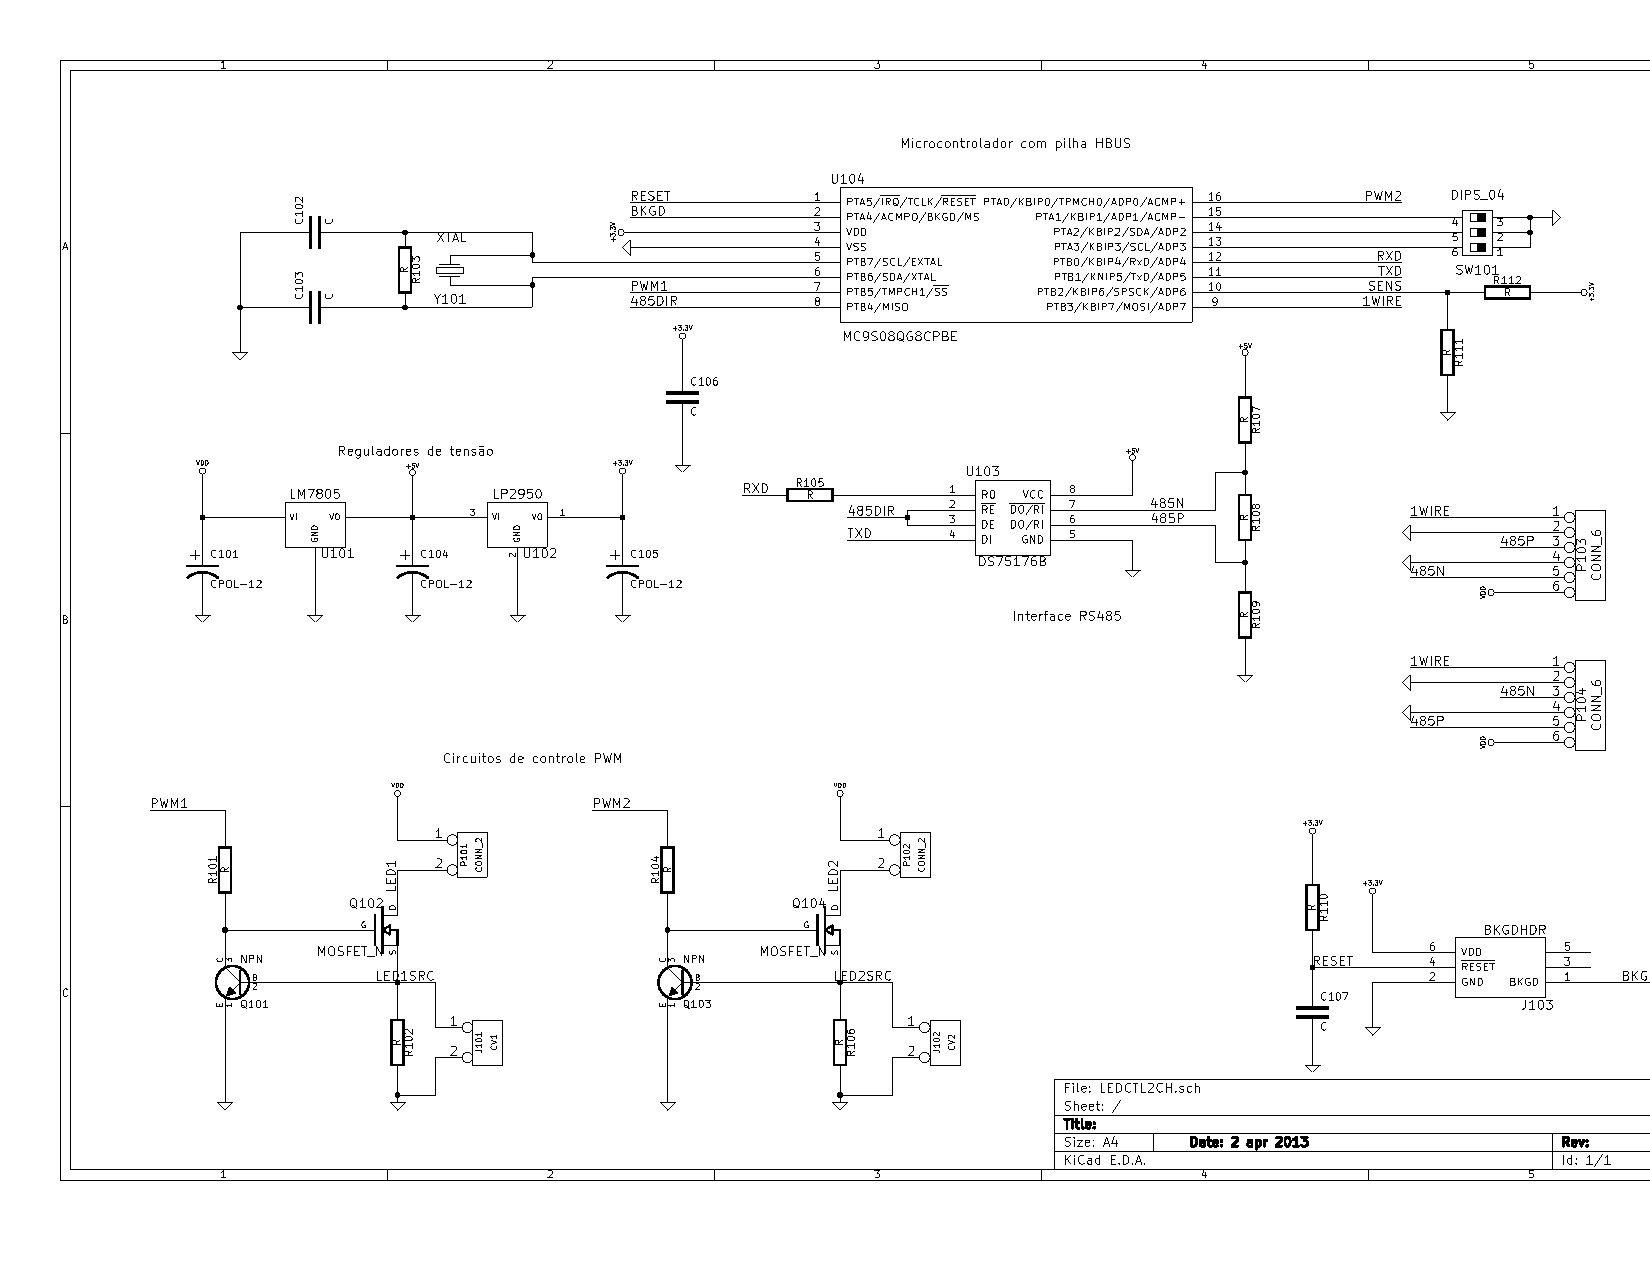
\includegraphics[scale=0.75]{../media/LEDCTL2CH.pdf}
\caption{Esquemático Controlador PWM 2 canais}
\end{figure}
